\documentclass[a4paper,11pt]{report}

\author{Florian~Hirtz}
\title{DUMMY: Entwicklung einer Applikation für Mobiltelefone zur Vermittlung von Nachhilfe}

\usepackage[ngerman]{babel}
\usepackage[utf8]{inputenc}
%Linux
%\usepackage[latin1]{inputenc}
\usepackage{blindtext}
\usepackage{graphicx}

%minimale page header & footer
\usepackage{fancyhdr}
\pagestyle{fancy}
\setlength{\headheight}{14pt} 
\fancyhf{}
\fancyhead[C]{\nouppercase{\leftmark}}
\fancyfoot[C]{\thepage}

%Depth of sections
\setcounter{secnumdepth}{3}
\setcounter{tocdepth}{3}
\bibliographystyle{abbrv}

%links
\usepackage{hyperref}

\begin{document}
	\maketitle
	\tableofcontents
	
	
	%VORWORT
	\chapter{Vorwort}
	DummyText...
		\section{Motivation}
		DummyText...
		\section{Danksagungen}
		DummyText...
	
	%Einleitung
	\chapter{Einleitung}
		\section{Zielsetzung}
		DummyText...
	
	%Konzeptionelle Grundlagen
	\chapter{Konzeptionelle Grundlagen}
		\section{Client-Server Prinzip}
		Das Client-Server Prinzip ist ein weit verbreitetes Konzept, um die Aufgaben innerhalb eines Netzwerkes effizient aufzuteilen. Dabei werden die Aufgaben auf zwei im Netzwerk agierenden Programme aufgeteilt. Diese Programme werden allgemein als Client und Server bezeichnet.
	 
		Der \emph{Server} hat die Aufgabe, verschiedenste Dienste zur Verfügung zu stellen, welche auf Anfrage ausgeführt werden können. Ein solcher Dienst kann zum Beispiel das Versenden einer Nachricht oder das Aufrufen einer Website sein. Der Server selbst ist passiv. Ein Server sollte immer in der Lage sein, Anfragen entgegenzunehmen und zu verarbeiten.
	
		Der \emph{Client} selber ist die aktive Komponente des Systems. Er ist in der Lage, Anfragen an den Server zu stellen und von dessen Diensten Gebrauch zu machen.
		Grundsätzlich gibt es in einem solchen Netzwerk nur einen Server, jedoch durchaus mehrere Clients. Ein guter Server sollte also auch darauf vorbereitet sein, mehrere Anfragen von verschiedenen Clients parallel zu bearbeiten. \cite{fachadmin.de:ServerClient}
		
		%TODO BILD VON SCHEMA SERVER-CLIENT
	
	%Projektentwicklung
	\chapter{Projektentwicklung}
	DummyText...
		\section{Systemüberblick}
		DummyText...
		
		%Die Server
			\section{Datenbank Server}
			Eine der wohl wichtigsten Aufgaben von Computern ist das Speichern, Verwalten und auch Manipulieren von Informationen. Anwendungen, die sich hauptsächlich mit dieser Aufgabe beschäftigen werden allgemein als \emph{Datanbanken} bezeichnet. Sie haben die Aufgabe, Informationen systematisch zu ordnen, zu speichern und bei Bedarf zu verändern. Grundsätzlich bezeichnet der Begriff Datenbank gleich zwei Dinge auf einmal. Zum einen wird ein strukturierter Speicher von Informationen als Datenbank bezeichnet und zum anderen jedoch auch die Anwendung, die das Verwalten der Daten überhaupt erst ermöglicht. Solche Anwendungen werden auch als \emph{Database Management System} (DBMS) bezeichnet und sind meist hochkomplex in ihren Funktionsweisen. \cite{IT-Handbuch}
			
			Datenbanken selbst wiederum können in  verschiedene Typen eingeteilt werden, die alle ihre eigenen Vor- und Nachteile mit sich bringen. Die einfachste Form eines Datenbanktyps ist wohl die \emph{Einzeltabellendatenbank}. Sie besteht aus nur einer Tabelle, in welcher alle Informationen abgespeichert werden. Sie eignet sich gut für kleine, übersichtliche Tabellenstrukturen wie zum Beispiel eine einfache Liste von Adressen. Die Einzeltabellendatenbank stösst jedoch spätestens dann an ihrer Grenzen, wenn die Informationen nicht mehr in nur einer, sondern gleich mehreren Tabellen gespeichert werden. Hier tritt ein anderer Datenbanktyp ins Spiel. Die \emph{relationale Datenbank}. Sie ist in der Lage, verschiedene Tabellen logisch miteinander zu verknüpfen und sich darin zu orientieren. Diese logische Verknüpfung ist möglich aufgrund eindeutigen Eigenschaften eines Eintrags. Dies kann zum Beispiel eine Kundennummer oder ein Name sein. Ein solches Feld wird auch als ein \emph{Key} bezeichnet. Wichtig dabei ist, dass jeder Key nur einmal in einer Tabelle vorkommt, ansonsten kann es Probleme bei der Verknüpfung kommen.\cite[S. 745 - 751]{IT-Handbuch}

				\subsection{MySQL Datenbank}
				%TODO GLOSSARY WORK ON LICENCE
				Ein Beispiel für ein solches \emph{Relational Database Management System} (RDBMS) ist die weit verbreitete MySQL Datenbank. Das System wurde ursprünglich von den drei Gründern Allan Larsson, Michael Widenius und David Axmark 1995 entwickelt und wurde später von \emph{Sun Microsytems} aufgekauft und gelangte schlussendlich in den Besitz von dem amerikanischen Softwarehersteller \emph{Oracle}. MySQL ist unter einem dualen Lizenzsystem eingetragen, sodass die Software zum einen unter einer \emph{General Public Licence} (GPL), aber auch unter eine proprietäre Lizenz gestellt ist. \cite{tecmint.com} Das MySQL System darf aufgrund der GPL gratis heruntergeladen, installiert und modifiziert werden. In Kombination mit der Programmiersprache PHP bildet sie eines der meist verwendeten Datenspeichersystemen für Webservice alles Art. Im Falle eines solchen Webservices befindet sich die Datenbank meist auf einem zentralen Server, auf welchem sich ebenfalls die benötigten PHP-Skripte befinden. Die PHP-Skripte haben die Aufgabe, Abfragen von den Clients entgegenzunehmen und über sogenannte \emph{Queries} (Datenbank Abfragen) auf die Informationen in der Datenbank zuzugreifen. Im falle einer MySQL Datenbank werden solche Queries in der Datenbanksprache \emph{SQL} formuliert. Queries können in vier Arten von Abfragen unterteilt werden: \cite[S. 760]{IT-Handbuch}
				
				\begin{itemize}
					\item Auswahlabfragen (\emph{Select Queries}) geben den Inhalt von einem oder mehreren Feldern aus einer oder verschiedenen Tabellen zurück. Dabei kann bei bedarf nach Kriterien gefiltert werden um die Suche nach bestimmten Datensätzen einzugrenzen.\cite[S. 746]{IT-Handbuch}
					\item Einfügeabfragen (\emph{Insert Queries}) fügen einen neuen Datensatz zu einer bestehenden Tabelle hinzu.\cite[S. 746]{IT-Handbuch}
					\item Änderungsabfragen (\emph{Update Queries}) ändern bestimmte oder alle Felder eines bereit bestehenden Datensatzes in einer Tabelle.\cite[S. 746]{IT-Handbuch}
					\item Löschabfragen (\emph{Delete Queries}) löschen einen Datensatz aus einer Tabelle. \cite[S. 746]{IT-Handbuch}
				\end{itemize}
				
				\subsection{MySQL Datenbankstruktur} \label{databankstructure}
				
				\begin{figure}
					\begin{center}
						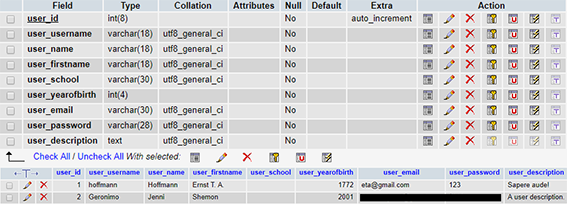
\includegraphics{user_archive.png}
						\caption{Die user\_archive Tabelle.}
						\label{user_archive:PNG}
					\end{center}
				\end{figure}
				\begin{figure}
					\begin{center}
						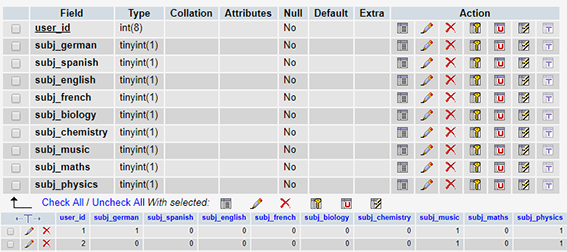
\includegraphics{user_subjects.png}
						\caption{Die user\_subjects Tabelle.}
						\label{user_subjects:PNG}
					\end{center}
				\end{figure}
				\begin{figure}
					\begin{center}
						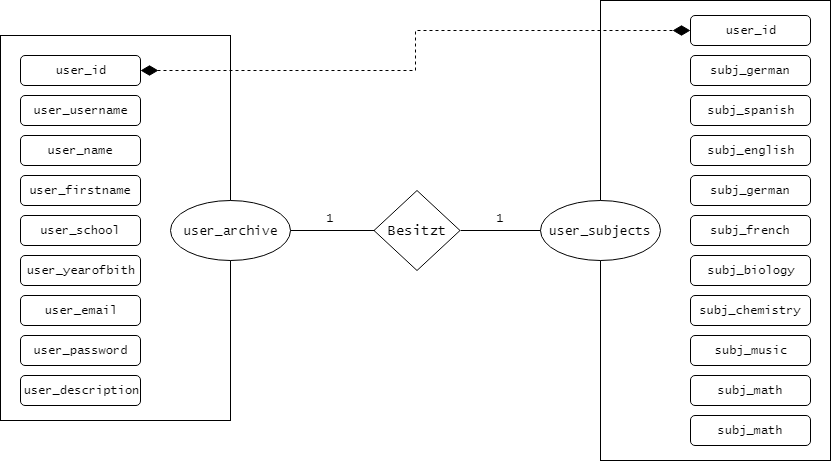
\includegraphics[width=0.8\textwidth]{ERM-Matura.png}
						\caption{Das ERM der entwickelten Applikation.}
						\label{ERM}
					\end{center}
				\end{figure}
				
				In der entwickelten Applikation wird genau ein solches MySQL Datanbanksystem in Kombination mit PHP (siehe Kapitel \ref{ssec:PHP})benutzt. Die Datenbank wird verwendet, um die Accountdaten der einzelnen Benutzer zu speichern und den Clients zur Verfügung zu stellen. Sie befindet sich auf dem Schulserver vom Ergänzungsfach. Die Datenbank selber umfasst zwei miteinander verknüpfte Tabellen. Die eine läuft unter dem Name \emph{user\_archive} (siehe Abbildung \ref{user_archive:PNG})und beinhaltet die essentiellen Accountdetails wie Name, Email, Passwort etc. Zu erwähnen ist hier das erste Feld \emph{user\_id}. Es wird bei einem neuen Eintrag in die Tabelle automatisch generiert (\emph{auto\_increment}) und gewährt so, dass sämtliche Einträge eindeutig unterschieden werden können. Ähnlich verhält sich das Feld user\_username. Es ist als \emph{unique} markiert und soll ebenfalls verhindern, dass es beim Login zu Mehrdeutigkeiten kommt. Sie sind die Keys der Tabelle. Die zweite Tabelle der trägt den Namen \emph{user\_subjects} (siehe Abbildung \ref{user_subjects:PNG}). Sie umfasst nebst einem Feld für die user\_id sämtliche momentan von der Applikation unterstützten Fächer. In den Feldern wird nun mithilfe von 1 und 0 angegeben, welche Fächer von einem Benutzer/ einer Benutzerin angewählt wurden, also in welchen er/sie andere unterstützen könnte. Die Inhalte wurden bewusst von einander getrennt, um die Übersichtlichkeit in der user\_archive Tabelle zu wahren. Das user\_id Feld ist auch hier ein Key und ist für jeden Benutzer gleich wie in der user\_archive Tabelle. Diese Verknüpfung der Tabellen kann sehr übersichtlich durch ein \emph{Entity-Relationship-Modell} (ERM) dargestellt werden, da das Modell lediglich zwei Tabellen (Im falle des ERM \emph{Entities}) umfasst. ERMs eignen sich besonders für die Darstellung von Datenbankstrukturen und deren Verknüpfungen. Sie sind oft der erste Schritt, wenn es um die Planung einer neuen Datenbank geht. Die Beziehungen werden durch hauptsächlich zwei Variablen beschrieben, welche im Schema (x, y) dargestellt werden. Die Variable x gibt das Minimum an herrschenden Beziehungen mit anderen Entities vor. Die Variable y das Maximum. Die Variablen können entweder eine bestimmte Zahl wie 1 oder 0 sein oder sie können durch m/n verkörpert werden, stellvertretend für beliebig viele Beziehungen. Im falle des ERMs der entwickelten Applikation (siehe Abbildung \ref{ERM}) ist das eine (1,1) : (1,1) Beziehung. Das bedeutet, dass es in beiden Tabellen jeweils genau einen Eintrag für einen Benutzer gibt. \cite[S. 750]{IT-Handbuch}\cite{ERM}\cite{ERM2}


				
				%TODO GLOSSAR OBJEKTORIENTIERT
				\subsection{PHP Skripte} \label{ssec:PHP}
				Nebst dem Datenbanksystem selbst befinden sich ebenfalls diverse PHP Skripte auf dem Server. Sie sind in der Open-Source Skriptsprache PHP geschrieben. PHP ist ein rekursives Akronym für \emph{Hypertext Preprocessor} und ist eine speziell für Webprogrammierung entwickelte Programmiersprache welche zu den objektorientierten Programmiersprachen gehört. PHP wird hauptsächlich für die Programmierung innerhalb von Webservern verwendet und bietet den grossen Vorteil, dass Clientbenutzer zwar durchaus die Skripte auf dem Server ausführen, jedoch nicht ansehen können. Sie erhalten lediglich eine Antwort ohne je die Codestruktur des PHP Skriptes zu Gesicht bekommen zu haben \cite{PHP}. Dies ist möglich, da dar PHP-Code ausschliesslich serverseitig ausgeführt wird. Ein \emph{Interpreter} führt ihn auf dem Server aus und erst die vom Interpreter generierte Ausgabe wird dem Client als Antwort zugeschickt. Die Antwort ist meist in der Auszeichnungssprache HTML (\emph{Hypertext Markup Language}) verfasst, können jedoch durchaus auch in PDF, JavaScript oder sogar Bildformaten sein.\cite{PHP:function}
				
				%TODO GLOSSAR PARSEN
				Die PHP-Skripte der Entwickelten Applikation verfassen alle ihre Antworten im Datenformat JSON (\emph{JavaScript Object Notation}).
				\begin{quotation}
					"JSON (JavaScript Object Notation) ist ein schlankes Datenaustauschformat, das für Menschen einfach zu lesen und zu schreiben und für Maschinen einfach zu parsen (Analysieren von Datenstrukturen) und zu generieren ist.[...]Bei JSON handelt es sich um ein Textformat, das komplett unabhängig von Programmiersprachen ist[...]. Diese Eigenschaften machen JSON zum idealen Format für Datenaustausch."\cite{JSON}
				\end{quotation}
				
					\subsubsection{Login}\label{login:php}
					Damit ein Client Zugriff auf einen Datensatz in der Datenbank bekommt, muss sich der Benutzer/ die Benutzerin zuerst unter einem bestehenden Account einloggen. Dabei wird auf dem Client Benutzername (Username) und Passwort eingegeben (siehe Kapitel \ref{login:act}). Daraufhin ruft der Client das \emph{login.php} Skript via Webadresse auf. Das aufgerufene Loginskript erstellt zuallererst eine Verbindung zur lokalen MySQL Datenbank. Daraufhin nimmt sie den Mitgeschickten Benutzernamen und das Passwort entgegen und speichert sie in lokalen Variablen. Als nächstes wird versucht ein Eintrag in der user\_archive Tabelle zu finden, bei welchem die Felder user\_username und user\_password mit den empfangenen Werten übereinstimmen. Dies wird über ein sogenanntes \emph{MySQL Statement} getan. In diesem Statement wird in der Datenbank nachgefragt, ob es einen Eintrag mit den bestimmten Angaben gibt (Select Query).
					\begin{quotation}
						{\fontfamily{qcr}\selectfont\noindent 'SELECT * FROM user\_archive WHERE user\_username=? AND user\_password=?'}
					\end{quotation}
				
					Wenn die Suche erfolgreich ist, wird auf das Statement mit dem Inhalt eines Datensatzes geantwortet, welcher dann vom PHP Skript wiederum lokalen Variablen zugewiesen wird. Nun ist auch die user\_id des Benutzers bekannt und es kann über ein zweites Statement den entsprechenden Datensatz aus der user\_subjects Tabelle ausgelesen werden. Wieder werden zurückgegebenen Werte in lokalen Variablen gespeichert. Die Werte aller gespeicherten Variablen werden nun in ein Array mit dem Namen \emph{response} übertragen und ihnen wird jeweils einen \emph{Key} (Zeichen, unter welchem der Wert im Array gespeichert ist) zugewiesen. Ebenfalls wird eine zusätzliche Variable unter dem Key \url{success} mit dem Wert \url{true} in den Array gespeichert. Die Variable \url{success} Teilt dem Client mit, dass die Anfrage erfolgreich war. Ist jedoch die Suche nach einem registrierten Benutzer mit eingegebenen Daten in der Datenbank erfolglos, verfasst das PHP Skript ein JSON Datei mit der Variable \url{response["success"] = false} und fügt keine weiteren Daten mehr an. Schlussendlich wird der Antwortarray mit den gespeicherten Daten in einem JSON Format gespeichert und das erstellte JSON File wird an den Client zurückgeschickt. Damit es beim Login zu keinen Mehrdeutigkeiten kommt ist es von Wichtigkeit, dass jeder Benutzername nur einmal in der Tabelle vorkommt (siehe Kapitel \ref{databankstructure}).
					\subsubsection{Registrierung}
					Wenn ein Benutzer/eine Benutzerin noch keinen Account hat, soll er/sie die Möglichkeit haben, sich einen zu erstellen. Hierzu kann er/sie auf dem Client die benötigten Daten eingeben (siehe Kapitel \ref{register:act}) und es wird eine Anfrage an das \emph{register.php} File auf dem Server geschickt. Das register.php Skript hat die Aufgabe, dem Benutzer einen Datensatz in beiden der Tabellen zu erstellen, sofern die Daten legitim sind. Zuerst wird dafür eine Verbindung mit der lokalen Datenbank aufgenommen. War dies Erfolgreich, wird daraufhin ein Auswahlabfrage formuliert, welche nach einem Datensatz mit dem eingegebenen Benutzernahmen fordert. Nur wenn kein solcher Datensatz gefunden werden kann, wird fortgefahren, ansonsten wird frühzeitig eine Antwort an den Client geschickt, die ihm mitteilt, dass die Registrierung Erfolglos war(siehe Kapitel \ref{login:php}). Wenn kein solcher Datensatz gefunden wurde, wird als nächstes ein Statement vorbereitet, welches einen neuen Datensatz in die Tabelle user\_archive einfügt (Insert Query), und bei welchem sogleich alle vom Benutzer/von der Benutzerin angegebenen Daten in die Felder eingefügt werden.
					\begin{quotation}
						{\fontfamily{qcr}\selectfont\noindent 'INSERT INTO user\_archive([...]) VALUES ([...])'}
					\end{quotation}
					
					Als nächstes soll noch einen Datensatz in der user\_subjects Tabelle eingetragen werden, welcher die gleiche user\_id hat, wie der soeben neu erfasste Datensatz in der user\_archive Tabelle. Hierzu wird zuerst über ein Statement die von der Datenbank automatisch zugewiesene user\_id aus der user\_archive Tabelle ausgelesen. Daraufhin wird eine weitere Insert Query mit der ausgelesenen ID und dem Wert 0 für alle Fächer in die user\_subjects Tabelle gestellt. Der Wert 0 steht in den Feldern stellvertretend für den Wert \url{false}, da neu erstellte Accounts per Default keine Fächer ausgewählt haben sollen. Schlussendlich, wird eine JSON Response verfasst, welche dem Client eine erfolgreiche Registrierung mitteilt.
					\subsubsection{Änderungen via Einstellungen vom Client}
					Es soll den Benutzern/Benutzerinnen möglich sein, gewisse Angaben wie Email, Passwort oder die Ausgewählten Fächer nachträglich zu verändern. Der Client bietet dafür eine Settings Activity (siehe Kapitel \ref{settings:act}) mit welcher die Angaben editiert werden können. Wenn die editierten Angaben auf dem Client gespeichert werden, wird eine Anfragen an das \emph{savesettings\_pw.php} File geschickt. Diese Skript soll die bereits bestehenden Datensätze auf der Datenbank verändern und die veränderten Daten zurückschicken. Hierzu wird zuerst eine Verbindung mit der Datenbank aufgenommen. Daraufhin wird überprüft, ob die Anfrage auch die Berechtigung für eine solche Änderungsabfrage (Update Query) hat. Im falle der entwickelten Applikation ist das sehr simpel gelöst. Es wird ähnlich wie beim login.php Skript eine Auswahlabfrage formuliert, die nach einem Datensatz mit einer bestimmten user\_id und Passwort fragt. Das Passwort muss vom Nutzer nicht manuell eingegeben werden, sondern wird im Hintergrund von der Client Applikation automatisch geregelt. Diese Vorkehrung ist aus Sicherheitsgründen sehr wichtig. Sollte das Passwort nicht überprüft werden, wäre es möglich, dass unberechtigte Personen die Datensätze von Benutzern/Benutzerinnen editieren könnten. Ist die Auswahlabfrage erfolgreich, wird zunächst eine Update Query formuliert, welches den Datensatz in der user\_archive durch den neuen mit den Aktualisierten Daten ersetzt.
					\begin{quotation}
						{\fontfamily{qcr}\selectfont\noindent 'UPDATE user\_archive SET [...] WHERE user\_id=?'}
					\end{quotation}
					
					Anschliessend wird der Datensatz per Auswahlabfrage wieder Ausgelesen und die Daten in lokalen Variablen gespeichert. Nun wird das gleiche mit der user\_subjects Tabelle gemacht. Zuerst eine Änderungsabfrage und daraufhin eine Auswahlabfrage. Sämtliche gespeicherten Daten werden in einen Array gespeichert und diese anschliessend im JSON Format an den Client zurückgeschickt.
					\subsubsection{Suchanfrage} \label{sssec:Suchanfrage}
					Damit es Benutzern/Benutzerinnen möglich ist, nach anderen Benutzern und Benutzerinnen zu suche, wird ein PHP Skript benötigt, welches die Datenbank nach Datensätzen durchsucht, welche bestimmten Kriterien unterliegen. Diese Kriterien kann der Benutzer/die Benutzerinnen auf dem Client angeben (siehe Kapitel \ref{filter:act}). Es soll nach Namen und nach Fächern gesucht werden können. Das search.php File übernimmt diese Aufgabe. Hierzu wird zuerst eine Verbindung mit der Datenbank aufgebaut. Ist das erfolgreich wird begonnen ein Statement zu formulieren, welches später als eine Select Query gestellt werden soll und alle den Kriterien entsprechenden Datensätze zurückliefern soll. Das MySQL Statement wird in zwei Schritten erstellt.
					
					Im ersten wird ein \emph{String} erstellt der gleich zwei Dinge tut. Zum einen schafft er eine Verknüpfung zwischen den beiden Tabellen user\_archive und user\_subjects. Dies wird durch die SQL Funktion \emph{INNER JOIN} erreicht.
					Diese Funktion ermöglicht es, die beiden Tabellen über die user\_id (Key) zu verbinden. Nun kann die Select Query in beiden Tabellen gleichzeitig nach mehreren Kriterien suchen und die Ergebnisse direkt zusammenführen.
					\begin{quotation}
						{\fontfamily{qcr}\selectfont\noindent 'SELECT user\_archive.*, user\_subjects.* 
							
						\noindent FROM user\_archive INNER JOIN user\_subjects ON
						
						\noindent user\_archive.user\_id = user\_subjects=user\_id [...]'}
					\end{quotation} 
					Zum anderen ist im String auch bereits das Suchkriterium bezüglich des Namens enthalten. Dazu wird die SQL Funktion \emph{LIKE} verwendet. Diese Funktion ermöglicht es, das nach Daten gesucht wird, die den eingegebenen Wert enthalten, jedoch nicht unbedingt komplett identisch sind. Zum Beispiel würde bei der Suche nach einem \glqq Max\grqq{} auch der Datensatz von \glqq Maximilian\grqq{} gefunden werden. Dies ermöglicht es Benutzern/Benutzerinnen auch ein gewünschtes Suchresultat zu finden, wenn sie nicht den ganz genauen Namen kennen.
					
					Im zweiten Schritt werden an den erstellten String noch die Kriterien für die ausgewählten Fächer angehängt. Dabei werden alle ausgewählten Fächer nacheinander als ein obligatorisches Kriterium an den String angehängt. Das bedeutet, dass wenn nach einer \glqq Magalie\grqq{} gesucht wird und gleichzeitig noch Mathematik als ein Kriterium ausgewählt ist, werden nur die Datensätze ausgewählt, bei welchen zum einen der Name \glqq Magalie\grqq{} vorkommt, aber auch Mathematik als ein Fach angegeben haben.
					
					Sind diese beiden Schritte erledigt, wird der String als eine Query ausgeführt und es werden die Datensätze zurückgegeben, die den Suchkriterien unterliegen. Nun werden die Informationen der Suchergebnisse mit Ausnahme des Passwortes zuerst einzeln in eigene Arrays gespeichert. Diese Arrays stellen sozusagen die einzelnen Suchergebnisse dar. Nun werden alle diese Arrays durchnummeriert in einen weiteren Array gespeichert. So sind alle Suchergebnisse kompakt und systematisch geordnet und können als ein einzelnes Element im Antwortarray referenziert werden. Nun wird noch der Wert \url{true} mit dem Key \url{"success"} im Antwortarray gespeichert und das ganze als JSON Datei dem Client zurückgeschickt.
					
					
			%TODO GLOSSAR API
			\section{Firebase}
			Firebase ist eine  Entwicklungsplattform für Webapplikationen, welche seit 2014 von Google Entwickelt wird. Firebse entwickelte sich aus dem 2011 gegründete Startup \emph{Envolve} von den beiden Gründern James Tamplin und Andrew Lee. Das Ziel von Envolve war es, Kunden eine API (\emph{Application Programming Interface}) zu bieten, mit welcher Realtime Chatfunktionen einfach realisiert werden können. Nachdem jedoch viele der Benutzer die API für noch viel mehr als nur Chats verwendeten, ja sogar einzelne Spielentwickler sie für eine Realtime Synchronisation verschiedener Clients verwendeten, begann die Entwicklung sich viel mehr auf das Anbieten einer API für Realtime Service zu konzentrieren. Der Erfolg war gross und 2014 wurde Google darauf aufmerksam und Kaufte das Unternehmen auf. Google entwickelte aus Envolve daraufhin eine Plattform, welche verschiedenste Tools zur Webserviceentwicklung anbietet und heute unter Namen Firebase bekannt ist. Firebase bietet sowohl Tools für die Entwicklung neuer Service wie Realtime Datenbanken, Authentifizierungsfunktionen und Crashanalysen, aber auch für das Unterhalten von bestehenden Servicen. Die Tools dürfen in einem begrenzten Rahmen gratis verwendet werden und sind daher sehr attraktiv für kleinere Entwicklerunternehmen.\cite{Firebase}
				\subsection{Firebase Realtime Datenbank}
				Wie bereits erwähnt, bietet Firebase unter anderem auch Realtime Datenbankfunktionen. Die Firebase Realtime Datenbank (RTDB) ist eine NoSQL Datenbank und unterscheidet sich in ihrer Funktionsweise stark von relationalen Datenbanken. Anders als relationale Datenbanken agieren Echtzeitdatenbanken nicht nur Passiv auf Anfrage, teilen den Clients aktiv mit, wenn sich ein Datensatz verändert hat (Push-Based Data Access) und halten ihn so immer auf dem neusten Stand. Echtzeitdatenbanken werden besonders dann eingesetzt, wenn sich ein Datensatz häufig oder jederzeit ändern kann und es von nöten ist, dass die Clients ohne grosse Verzögerung davon unterrichtet werden.\cite{RealtimeDatabase} Es ist dann nicht einmal nötig, das die Clients zur zeit des Pushes online sind. Sie werden bei Start automatisch mit dem Datensatz auf der Datenbank abgeglichen und aktualisiert.\cite{FirebaseRTDB}
				
				Die Chatfunktion in der entwickelten Applikation ist ein genau solcher Service, der einen solche Datenbank benötigt. So können Clients in Echtzeit via untereinander Kommunizieren ohne das sie entweder permanent online sein müssen, oder konstant die Applikation neu laden müssen. Die Wahl für die Firebase Plattform ist dann einfach gewesen. Der Client ist im ebenfalls von Google entwickelten Android Studio entwickelt worden. Android Studio Unterstützt per default die Firebase API, weshalb das Einbinden einer Firebase RTDB in eine Applikation sehr simpel ist (siehe Kapitel \ref{chat:act}).
				\subsection{Firebasestruktur}
				Firebase Echtzeitdatenbanken haben eine andere Struktur als relationale Datenbanken. Die Informationen sind nicht in Form von Tabelle gespeichert sondern kann vielmehr mit der Struktur eines Ordnersystems verglichen werden. Die Informationen werden unter einer Form von Ordnern gespeichert und in einem System geordnet. Der Ort, wo die Informationen gespeichert sind, wird in Pfaden angegeben, die mit denen von einem Filesystem eines Computers zu vergleichen sind. Dabei gibt es einen Hauptordner, der Sozusagen die gesamte Datenbank umfasst. Diese wiederum hat Unterordner, welcher allgemein als \emph{Children} bezeichnet werden.
				
				Die Struktur der verwendeten Datenbank kann grundsätzlich in zwei Ordner aufgeteilt werden. Der \emph{User}-Ordner und der \emph{Chats}-Ordner. Im User Ordner	sind alle Benutzer verzeichnet, die einen oder mehrere offene Chats besitzen. Der Ordner ist hauptsächlich dazu da, um die offenen Chats eine Benutzers auf der Hauptseite des Clients darstellen und öffnen zu können. Die Children des Verzeichnis sind unter den IDs der Benutzer gespeichert. Für jeden offenen Chat findet sich in einem Solcher Child nun ein weiteres Child für jeden offenen Chat des Benutzers/der Benutzerin. Dieses enthält nun die eigentlichen Informationen, die für das Öffnen und darstellen des Chats benötigt werden. Ebenfalls enthalten sie auch den Pfad des eigentlichen Chats, wo auch die Nachrichten gespeichert sind (siehe auch Kapitel \ref{warum}). Die offenen Chats findet man alle im Chats Verzeichnis. Dort sind als Children alle Chats zu finden. Der Name wird ihnen durch die beteiligten Chatpartner/Chatpartnerinnen gegeben. Das heisst, ein Chat zwischen der Benutzer A mit der ID 9 und einer Benutzerin B mit der ID 21 würde unter dem Namen 9>>21 zu finden sein. Im Chatverzeichnis selber befinden sich alle gesendeten Nachrichten. Der Name der Nachrichten wird von Firebase selber generiert. Die Nachrichten enthalten nun die drei eigentlich versendeten Werte: die Nachricht, das Sendedatum und Uhrzeit und der Absender/die Absenderin.
				
				\subsubsection{Warum genau diese Struktur?} \label{warum}
				Es ist an dieser Stelle vielleicht noch interessant zu erwähnen, weshalb die Firebasestruktur auf den ersten Blick etwas überkompliziert erscheinen mag. Der Grund dafür ist nämlich eine Eigenheit von Echtzeitdatenbanken. Anders als bei relationalen Datenbanken ist es in Echtzeitdatenbanken nur schwer möglich, nach Einträgen zu Suchen, bei welchen nicht der gesamte Namen bekannt ist. Somit ist es nicht möglich für die Darstellung der Chats auf der Hauptseite einfach nach Einträgen im Chats Ordner zu suchen, in welchen die ID des Benutzers/der Benutzerin vorkommt. Deshalb musste eine Alternative gefunden werden, welche sich nun in der Form des User Ordners ausdrückt. Dort werden nämlich alle Pfade zu den Chats gespeichert, in welchen ein Benutzer/eine Benutzerin vorkommt. Die Pfade werden beim eröffnen eines neuen Chats dort eingetragen. Auf diese Weise ist es trotzdem möglich, alle offenen Chats eines Benutzers/einer Benutzerin Anzuzeigen, ohne das eine Suchfunktion dafür benötigt wird.
		%Der Client
		\section{Client}
		Der Client ist das Herzstück des Service. Er ist der, der schlussendlich bei den Endbenutzern/Endbenutzerinnen heruntergeladen und benutzt wird. Er ist das Verbindende Glied zwischen den gespeicherten Informationen auf dem Server und den Benutzern/Benutzerinnen. Der Client, welcher im Rahmen dieser Arbeit entwickelt wurde, ist für Android Geräte programmiert worden. Er wurde in der Programmierumgebung \emph{Android Studio} entwickelt. Android Studio ist ein von Google entwickelter IDE für die Entwicklung von Java Applikationen für Android Mobilgeräte. Der IDE bietet diverse hilfreiche Tools für Entwickler wie das erstellen von virtuellen  Geräten für das sichere Testen der Applikationen oder eine Umgebung für das gestalten von User Interfaces. Somit viel die Wahl für die Entwicklung diese Applikation sehr schnell auf Android Studio, da die Umgebung so gut wie alles besitzt, was für die Entwicklung einer solchen Applikation gebraucht wird.
			\subsection{Programmiersprache}
			Die Applikation wurde vorwiegend in der Programmiersprache Java verfasst. Java ist eine Sprache der 3. Generation und gehört zu den objektorientierten Programmiersprachen. Sie wurde erstmals 1995 von Sun Microsystems veröffentlicht und ist nun seit 2010 in Besitz von Oracle. Java zeichnet sich besonders durch seine Plattformunabhängigkeit aus und eignet sich daher besonders gut für kleinere Applikationen, die auf vielen verschiedenen Geräten gleich funktionieren sollen. Das Betriebssystem Android, für welche die Applikation entwickelt worden ist, ist das Weltweit meist verwendete OS für Mobiltelefone und unterstützt standardmässig die auf Java basierte Laufzeitumgebung \emph{Android Runtime}. Somit werden fast alle Applikationen für Android in der Sprache Java entwickelt, weshalb auch der Client dieser Arbeit in Java geschrieben wurde, um eine möglichst grosse Menge an Benutzern/Benutzerinnen zu erreichen.\cite{android}
			\subsection{Architektur des Clients}
			Der Client der Applikation besteht aus insgesamt zehn sogenannten \emph{Activities}. Activities sind sozusagen die verschiedenen Fenster die in einer Applikation geöffnet werden können. Eine Übersicht über alle Activites findet sich auf der nächsten Seite. Activities sind grundsätzlich in zwei Komponenten aufgeteilt. Zum einen die \emph{View}-Komponente welche in der Layoutsprache XML geschrieben ist und das Userinterface der Activtiy bestimmt. Die zweite Komponente ist die dazugehörende \emph{Controller}-Klasse, welche in Java ist programmiert ist.
				
				\subsubsection{Klassenübersicht}
				Nebst den Activities und ihren jeweiligen Controller sind auch noch eine Reihe von anderen Klassen verwendet worden.
				\paragraph{Die Request Klassen}
				Für die Anfragen an den Server werden Request-Klassen verwendet. Sie sind Children von der Klasse \emph{Stringrequest} und erstellen aus den zu versendenden Daten eine lokale Hashmap. Die Request Klasse beinhaltet ebenfalls die URL des PHP-Files, an welches die Anfrage gesendet werden soll. Die Request-Klassen können da sie Children der Stringrequest Klasse sind in sogenannten \emph{Request Queues} dann ausgeführt werden. Die für diese Aufgabe verwendeten Funktionen finden sich alle in der \emph{Volley} Library. Volley bietet diverse Tools für das effiziente arbeiten mit Netzwerken und eignet sich daher perfekt für die Aufgabe.\cite{volley}
				\paragraph{Die Adapter Klassen}
				Adapter Klassen sind bestimmend für das Verhalten von Auflistungen. Es gibt einen Adapter für die Anzeige der Suchergebnisse, den Chat und dem Bottomsheet von der Haupseite, wo die offenen Chats angezeigt werden. Adapter geben der Applikation vor, wie die verschiedenen Elemente einer Liste anzuzeigen sind. Für die Suchergebnisse wird dafür eine Child der Klasse \emph{Base Adapter} aus der \emph{Widget} Library verwendet. Die anderen beiden Adapter sind Children der \emph{Firebase Recycler Adapter} Klasse aus der Firebase Library. Sie sind für das Auflisten von Objekten in der Firebase Datenbank verantwortlich und haben jeweils eine Referenz zu einem Verzeichnis in der Firebase Datenbank, dessen Inhalt sie auflisten.
				\paragraph{Die userInfo und JSONtoInfo Klasse}
				Damit die einzelnen Activities nicht immer wieder von neuem Anfragen an den Server senden müssen, geben sie sich jeweils die Informationen untereinander weiter. So muss nur einmal zu beginn beim Login eine Anfrage statt finden. Die Informationen werden unter den Activitis im selben JSON String weitergegeben, wie sie vom Server empfangen wurden. Der String ist kompakt und kann in nur einer Linie jeweils weitergegeben werden. Er eignet sich jedoch nicht für den Gebrauch in den Activities selber. Hierzu gibt es die userInfo Klasse. Sie fungiert als eine Art \glqq Variabelcontainer\grqq{} und besitzt sämtliche Eigenschaften, die ein Benutzerprofil besitzt. Dazu gehört Namen, Fächer, Passwort etc. Diese gespeicherten Variablen können dann in den Activities an den angeforderten Stellen über sogenannte \emph{Getter}-Funktionen ausgelesen werden. Die JSONtoInfo Klasse wiederum besteht aus nur einer Funktion, die in der Lage ist, den JSON-String in eine Instanz der userInfo Klasse zu speichern. So wird also in jeder Activity zuerst aus dem JSON-String eine userInfo Klasse instantiiert, die nachher als für den Zugriff auf die Accountinformationen gebraucht werden kann.
			
			%Alle Module des Clients
			\subsection{Module}
				\subsubsection{Login Activity} \label{login:act}
				Der Login Screen ist der erste Screen, der ein Benutzer/eine Benutzerin zu Gesicht bekommt, wenn er/sie die Applikation startet. Er fordert den Benutzer/die Benutzerin auf, sein/ihr Benutzernamen und Passwort einzugeben. Das Design ist sehr allgemein gehalten und ist Vergleichbar mit dem vieler anderer Login Screens von diversen Applikationen. Über der Eingabe ist das Logo der Applikation zu sehen. Es soll das sonst sehr allgemeine Login etwas einzigartiger machen, um mit einem guten Logo dem Benutzer/der Benutzerin gleich in Erinnerung zu bleiben. Unter dem auffälligen Login Knopf findet sich der Link zum Registrierungsformular. Es ist bewusst unauffällig gestaltet, da jeder Benutzer es voraussichtlich nur einmal brauchen wird und es sonst das Bild stören würde. Das Design und der Text des Links sind inspiriert von anderen Loginformularen populärer sozialer Netzwerke wie Instagram oder Twitter. Sollte ein Benutzer/eine Benutzerin auf den Link klicken, öffnet sich die Register Activity (siehe Kapitel \ref{register:act}). Wenn auf den Login Knopf gedrückt wird, wird ein login\_request mit eingegebenem Benutzernamen und Passwort generiert und das login.php File auf dem Server aufgerufen (siehe Kapitel \ref{login:php}). Ist die Anfrage erfolgreich, wird der JSON String in in die \emph{Extras} (Datencontainer, mit welchem Werte zwischen Activities weitergegeben werden können) gespeichert und die Hauptseite gestartet(siehe Kapitel \ref{mainpage:act}).
				
				Der Controller des Logins besteht im wesentlichen aus 4 Komponenten. Der standard Methode \emph{onCreate}, die das XML Layout des Logins aufruft und gewisse Variablen instantiiert. diese Methode existiert bei allen Activities und wird später nicht mehr speziell erwähnt. Weiter gibt es noch die beiden \emph{Listenerklassen} für sowohl den Login Knopf wie auch das Label für die Registrierung. Sie bestimmen, was geschehen soll wenn auf diese Elemente gedrückt wird. Zuletzt gibt es noch die \emph{Responselistener} Klasse. Sie ist für das Verarbeiten der vom Server empfangenen Antwort verantwortlich. 
				\subsubsection{Register Activity} \label{register:act}
				Das Registrierungsformular fragt den Benutzer/die Benutzerin nach allen Informationen, die benötigt werden, um ihm/ihr einen eigenen Account zu erstellen, unter welchem sie sich einloggen kann. Dazu wird nach einem Benutzernamen, einem Vor- und Nachnamen, dem Geburtsjahr, der aktuell besuchten Schule, eine Email und einem Passwort gefragt. Zudem gibt es noch zuletzt eine Checkbox für die AGBs und einen Knopf um sich schliesslich zu registrieren. Wenn diese angewählt wird, wird zuerst geprüft, dass auch alle Felder richtig ausgefüllt sind. Ist das der Fall, wird ein register\_request vorbereitet und eine Anfrage an das register.php File auf dem Server geschickt. Teilt die Antwort einen Erfolg beim erstellen eines neuen Accounts mit, so wechselt der Bildschirm automatisch zurück zum Login Screen. Sollte ein Benutzer/eine Benutzerin trotz keiner erfolgreichen Registration zurück zum Login Screen wollen, so kann sie den Pfeil im linken oberen Ecken verwenden, welcher sie zurück auf die Login Seite bringt. Diese Pfeile sind mittlerweile Standard geworden innerhalb von Android wie aber auch IOS Applikationen. Da sich die Benutzer wahrscheinlich bereits an diese Funktion gewöhnt haben, wird sie auch innerhalb der Applikation mehrmals verwendet, um die Bedienung der Applikation möglichst natürlich und intuitiv zu gestalten.
				
				In der Controllerklasse finden sich die 5 Hauptkomponenten der Activity. Der Listener für den Registrier-Knopf, Der Responselistener für die Registrierung, die onCreate Methode, eine Methode für den Zurück-Knopf und noch eine Methode, die die letzen 100 Jahre in den Spinner einfügt, der benötigt wird, um den Jahrgang anzugeben. Die Methode für den Spinner ermöglicht es, dass die Applikation automatisch neue mögliche Jahrgänge einfügt und nicht manuell jedes neues Jahr eingetragen werden muss.
				\subsubsection{Mainpage Activity} \label{mainpage:act}
				Die \emph{Mainpage Activity} ist sozusagen das Herz der Applikation. Sie wird direkt nach erfolgreichem Login geöffnet und ist sozusagen das eigene Profil des Benutzers/der Benutzerin. Von hier aus können verschiedene Dinge gemacht werden. Zum einen kann man mithilfe eines Knopfes im rechten oberen Ecken in sie Einstellungen gelangen (siehe Kapitel \ref{settings:act}). Weiter kann über den Knopf im unteren rechten Bereich des Bildschirms die Suchfunktion der Applikation ausgeführt werden. Der Knopf soll möglichst offensichtlich platziert sein, damit der Benutzer/die Benutzerin ohne Probleme die Suchfunktion findet. Ebenfalls kann durch ein Ausfahrbares Bottomsheet auf offenen Chats zugegriffen werden. Das Profil selber besteht aus den Ausgewählten Fächern, welche ähnlich wie Medaillen dargestellt werden, einem später setzbaren Profilbild mit Name des Benutzers/der Benutzerin und einer Beschreibung.
				
				Der Controller der Mainpage beinhaltet die 6 Komponenten der Activity. Zum einen wider die onCreate Methode, die hier hauptsächlich die Informationen, welche vom Server empfangen wurden in die Felder einfügt. Weiter gibt es noch die beiden Listener Klassen für sowohl den Suchknopf wie auch für den Einstellungen Knopf. Dazu kommt noch ein weiterer Listener, der beschreibt, wie das Bottomsheet ausgefahren werden soll. Zuletzt kommt noch eine onStart und eine View Holder Klasse Methode. Die View Holder Klasse beschreibt lediglich, wie die einzelnen Viewkomponenten des Layouts des offenen Chats ausgefüllt werden sollen. Die onStart Methode ist ähnlich wie die onCreate Methode, ist hier jedoch vor für das Bottomsheet von Bedeutung. Sie weist dem Bottomsheet einen der bereits erwähnten Firebase Adapter zu und gibt die View Holder Klasse mit. Somit kann das Bottomsheet mit allen offenen Chats ausgefüllt werden. Die einzelnen offenen Chats bekommen ihre Listener Klassen vom Firebase Adapter und nich von der Mainpage Activty.
				\subsubsection{Settings Activity} \label{settings:act}
				Die Settings Activity teilt sich eigentlich in ganze 3 Activites auf, der \emph{settingsOverview Activity}, der \emph{profileSettings} Activity und der \emph{securitySettings} Activity. Die settingsOverview Activity ist lediglich ein Navigator. In ihr finden sich die beiden verweise zu den anderen Eintsellunsactivites. Dies ist vor allem bei Mobilapplikationen weit verbreitet. Da der Screen nur sehr beschränkten Platz zur Verfügung hat, werden volle Formulare schnell unübersichtlich. Dann lohnt es sich das Formular in verschiedene kleinere Formulare aufzuteilen, wie es auch hier gemacht worden ist. In der securitySettings Activty können dinge wie Passwort oder Email bearbeitet und anschliessend gespeichert werden. In der profileSettings Activity wiederum sind die Einstellungen bezüglich des Profils wie Name, Fächer und Schule zu finden. Wenn die Einstellungen beider Activies gespeichert werden wird ein savesettings\_pw\_request erstellt und an das savaestetting\_pw.php eine Anfrage geschickt. Bei Erfolg ändert der Screen automatisch zurück zu Übersicht.
				\subsubsection{Filter Activity} \label{filter:act}
				Die Filter Activity wird durch von der Hauptseite aus erreicht und ist dazu da, damit der Benutzer/die Benutzerin ihre Suchkriterien eingeben kann. Dazu gehört Name und Fach. Der Name kann optional in einem Textfeld eingegeben werden während die Fächer über Checkboxen ausgewählt werden können. Darunter findet sich ein Knopf, der die effektive Suche startet. Es wurde bewusst auf eine Dynamische Suchfunktion verzichtet, da sonst das einbauen des Filtern nach Fächern etwas unübersichtlich geworden wäre. Mithilfe diese Filter Activity können sich Benutzer/Benutzerinnen zuerst in ruhe ihre Suchkriterien auswählen und sich anschliessend in die Ergebnisse evaluieren. Beim drücken des Suchknopfes unter den Kriterien wird ein serach\_request erstellt, der eine Anfrage an das search.php File schickt. Wenn die Suche Ergebnisse liefert, wird die Searchresults Activity gestartet.
				
				Die Controler Klasse der Filter Activity besteht aus lediglich 4 Komponenten. Der onCreate Methode, der Methode für den Pfeil zurück zur Mainpage, eine Listener für den Suchknopf und noch einem ResponseListener.
				\subsubsection{Searchresults Activty}
				Die Searchresults Activity hat die Aufgabe, die vom Server gefundenen Suchergebnisse anzuzeigen. Das Layout der Activity selber besteht lediglich aus einer Liste. Spannender ist da das Layout der einzelnen Komponenten der Liste. Jede Komponente repräsentiert ein Suchergebnis und somit ein Profil eines Nutzers/einer Nutzerin. Die einzelnen Elemente sind so gestaltet, dass beim durch scrollen gleich alle wichtigsten Informationen herausgelesen werden können. Dazu gehören Namen, Geburtsjahr, Fächer und Profilbild. In die List einegefüllt werden die einzelnen Komponenten von einem Adapter, der jeweils das Layout bestimmt und den Informationen des Profils anpasst. Damit die einzelnen Elemente auch angewählt werden können, wird noch ein Listener benötigt, der den jeweiligen Elementen auch ein bestimmtes Profil zuweist und die Userprofile Activity starten kann. Diese wird in der Searchresults Activity selbst als ein Child der Klasse \emph{onItemSelectedListener} bestimmt. Wenn nun ein Element der Liste ausgewählt, so holt sich der Listener die Indexnummer, an welcher das Element steht. Dieser Index entspricht dem Index der Profilinformationen im erhaltenen Antwortarray (siehe Kapitel \ref{sssec:Suchanfrage}) und somit können die im Array gespeicherten Informationen über den Index an die Userprofile Activity weitergegeben werden.
				\subsubsection{Userprofile Activty}
				Die Userprofile Activity 
				\subsubsection{Chat Activity} \label{chat:act}
		
\newpage
\bibliography{literatur}	
	
\end{document}